\chead{Question 5} 




\begin{tcolorbox}
\textbf{Question 5} 
Given $f(x)=2-x^{2} \sin (x)$ has a solution in the interval $[-1,2]$.
\begin{enumerate}[label=(\alph*)]
	\item Sketch the graph for $f(x)$ on interval $[-10,10]$
	\item Apply five steps of Newton's Method with initial guess $x_{0}=-1$ to attempt to find this root.
	\item Apply five steps of Newton's Method with initial guess $x_{0}=2$ to attempt to find this root.
	\item Compare the results of (b) and (c), explain what happens.
\end{enumerate}

\end{tcolorbox}

\begin{solution}\ \\


\begin{enumerate}[label=(\alph*)]

\item
The Diagram generated by MatLab (\ref{Q5_a_1})\\
\begin{figure}[htb]
	\centering %图片居中
  	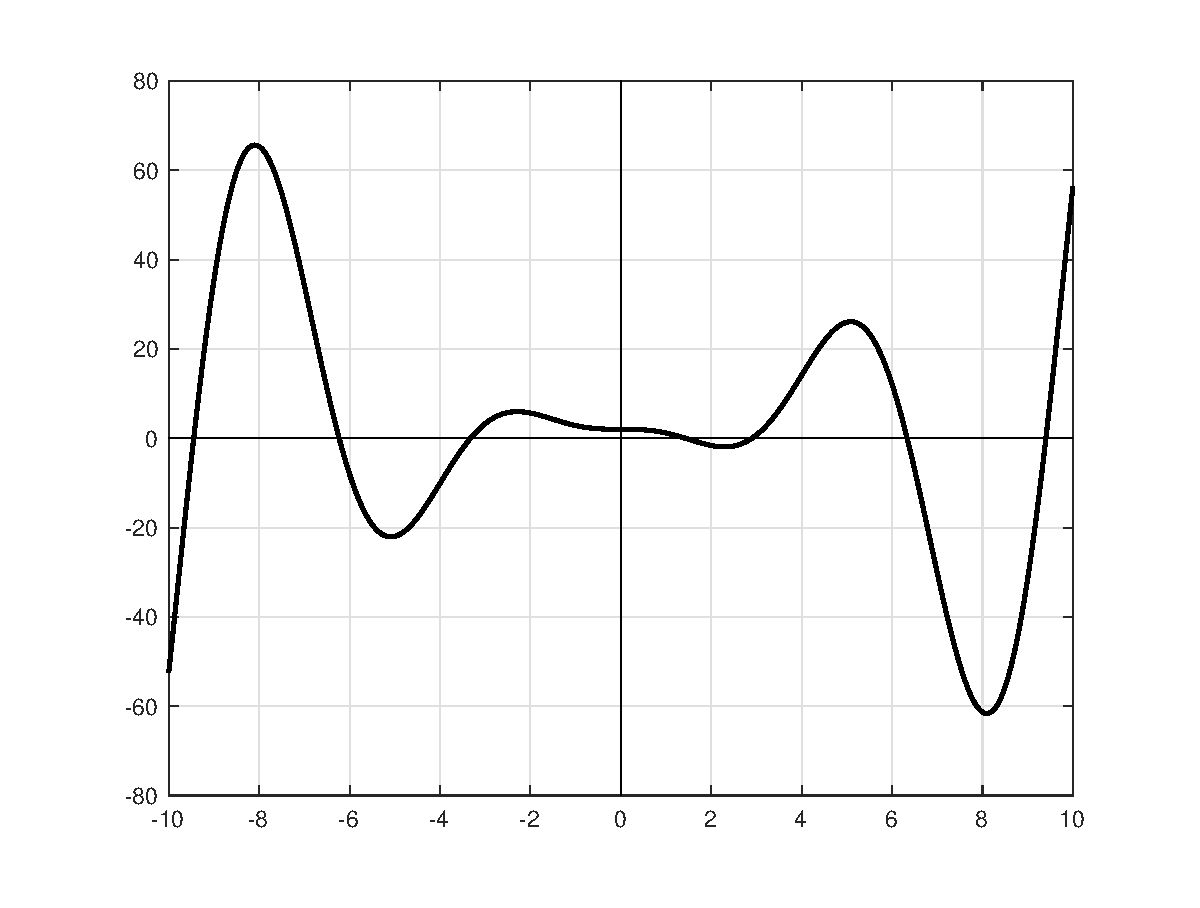
\includegraphics[width=0.7\textwidth]{fig/Q5_plot.eps}
  	\caption{(a) $f(x)=2-x^2 \sin(x)$} \label{Q5_a_1}
\end{figure}


\item Here first find the iteration method.\\

\begin{equation}
	x_{i+1}=x_{i}-\frac{f\left(x_{i}\right)}{f^{\prime}\left(x_{i}\right)} \label{Q5_iteration}
\end{equation}


Here the function is given that

\begin{equation}
	f(x)=2-x^2\sin (x) \label{Q5_equation}
\end{equation}

\begin{equation}
	f'(x)=-2x \sin(x) - x^2 \cos(x) \label{Q5_equation_derivative}
\end{equation}

Therefore input (\ref{Q5_equation}) and (\ref{Q5_equation_derivative}) into (\ref{Q5_iteration}),the function is given that:


\begin{equation}
	x_{i+1} =x_{i}-\frac{2-x_i^2\sin (x_i)}{-2x_i \sin(x_i) - x_i^2 \cos(x_i)} 
\end{equation}
	
	
In this section we set the initial guess, $x_0=-1$:



$$
x_{1} =x_{0}-\frac{2-x_0^2\sin (x_0)}{-2x_0 \sin(x_0) - x_0^2 \cos(x_0)}=0.2781
$$ 

$$
x_{2} =x_{1}-\frac{2-x_1^2\sin (x_1)}{-2x_1 \sin(x_1) - x_1^2 \cos(x_1)}=8.994
$$ 


$$
x_{3} =x_{2}-\frac{2-x_2^2\sin (x_2)}{-2x_2 \sin(x_2) - x_2^2 \cos(x_2)}=9.475
$$ 

$$
x_{4} =x_{3}-\frac{2-x_3^2\sin (x_3)}{-2x_3 \sin(x_3) - x_3^2 \cos(x_3)}=9.403
$$ 

$$
x_{5} =x_{4}-\frac{2-x_4^2\sin (x_4)}{-2x_4 \sin(x_4) - x_4^2 \cos(x_4)}=9.402
$$ 


\item

In this section we set the initial guess, $x_0=2$:

$$
x_{1} =x_{0}-\frac{2-x_0^2\sin (x_0)}{-2x_0 \sin(x_0) - x_0^2 \cos(x_0)}=1.170
$$ 

$$
x_{2} =x_{1}-\frac{2-x_1^2\sin (x_1)}{-2x_1 \sin(x_1) - x_1^2 \cos(x_1)}=1.445
$$ 


$$
x_{3} =x_{2}-\frac{2-x_2^2\sin (x_2)}{-2x_2 \sin(x_2) - x_2^2 \cos(x_2)}=1.422
$$ 

$$
x_{4} =x_{3}-\frac{2-x_3^2\sin (x_3)}{-2x_3 \sin(x_3) - x_3^2 \cos(x_3)}=1.422
$$ 

$$
x_{5} =x_{4}-\frac{2-x_4^2\sin (x_4)}{-2x_4 \sin(x_4) - x_4^2 \cos(x_4)}=1.422
$$ 


\item




Here we first plot the graph of the iteration point generated by 5(b) and 5(c), (\ref{Q5_d_1}):

\begin{figure}[htb]
\centering
\subfigure[5(b)]{
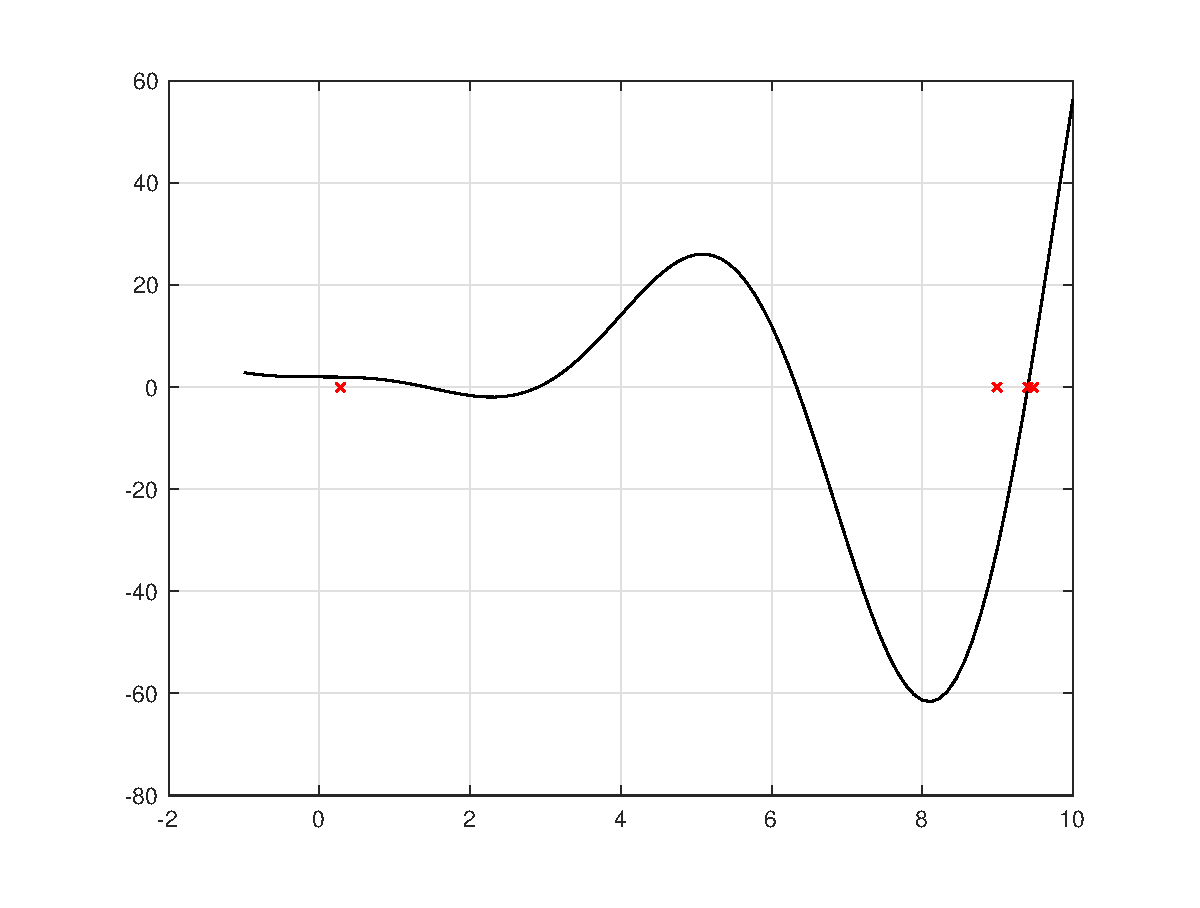
\includegraphics[width=7.5cm]{fig/Q5_d_1.eps}
%\caption{fig1}
}
\quad
\subfigure[5(c)]{
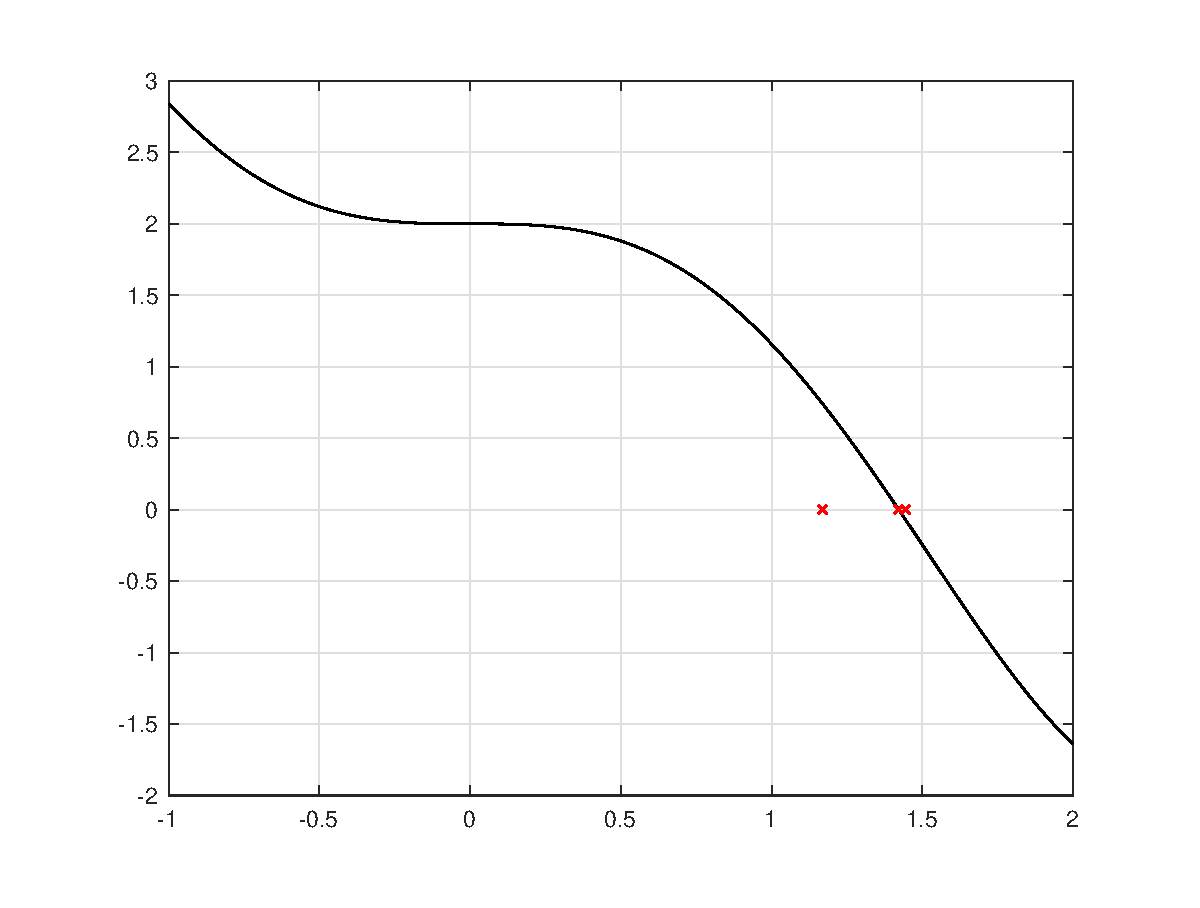
\includegraphics[width=7.5cm]{fig/Q5_d_2.eps}
}
\caption{Iteration Point of 5(b) and 5(c)}
\label{Q5_d_1}
\end{figure}



Therefore it is easy to find that in 5(b),the initial guess leads to the root jump to another region, out of the required range. Which is one of the drawback of the Newton's Method: In some cases where the function is oscillating and has a number of roots, one may choose an initial guess close to a root. However, the guesses may jump and converge to some other root.


Here we can plot the graph to illustrate the procedure of the root jumping in 5(b),(\ref{5_d_3}). Newton's Method could be described in figure that we choose one point and found the tangent line on $f(x)$, the focus of the tangent and X axis will be the result and the initial value of the next iteration. Here we hope the focus point can be closer to the root we want. 



\begin{figure}[htb] %H为当前位置,!htb为忽略美学标准,htbp为浮动图形
\centering %图片居中
\includegraphics[width=0.6\textwidth]{fig/Q5_d_3.eps} %插入图片,[]中设置图片大小,{}中是图片文件名
\caption{The procedure of the root jumping in 5(b)} %最终文档中希望显示的图片标题
\label{5_d_3} %用于文内引用的标签
\end{figure}







However in 5(b), when the second times of the iteration leads to an abnormal focus with the x axis. This is because in the local region, the slope is too small and turn to be flat (\ref{Q5_d_4}), which leads the focus locate in second iteration far from the required region, at $8.994375358445748$, and then the further iteration leads to converge to another root around $9.4$.


In 5(c) we start at $x_0=2$, here by plotting the graph of the derivative, we can find that the slope is enough to let the result converge to the root without jumping. (\ref{Q5_d_4})


\begin{figure}
\centering
\subfigure[5(b)]{
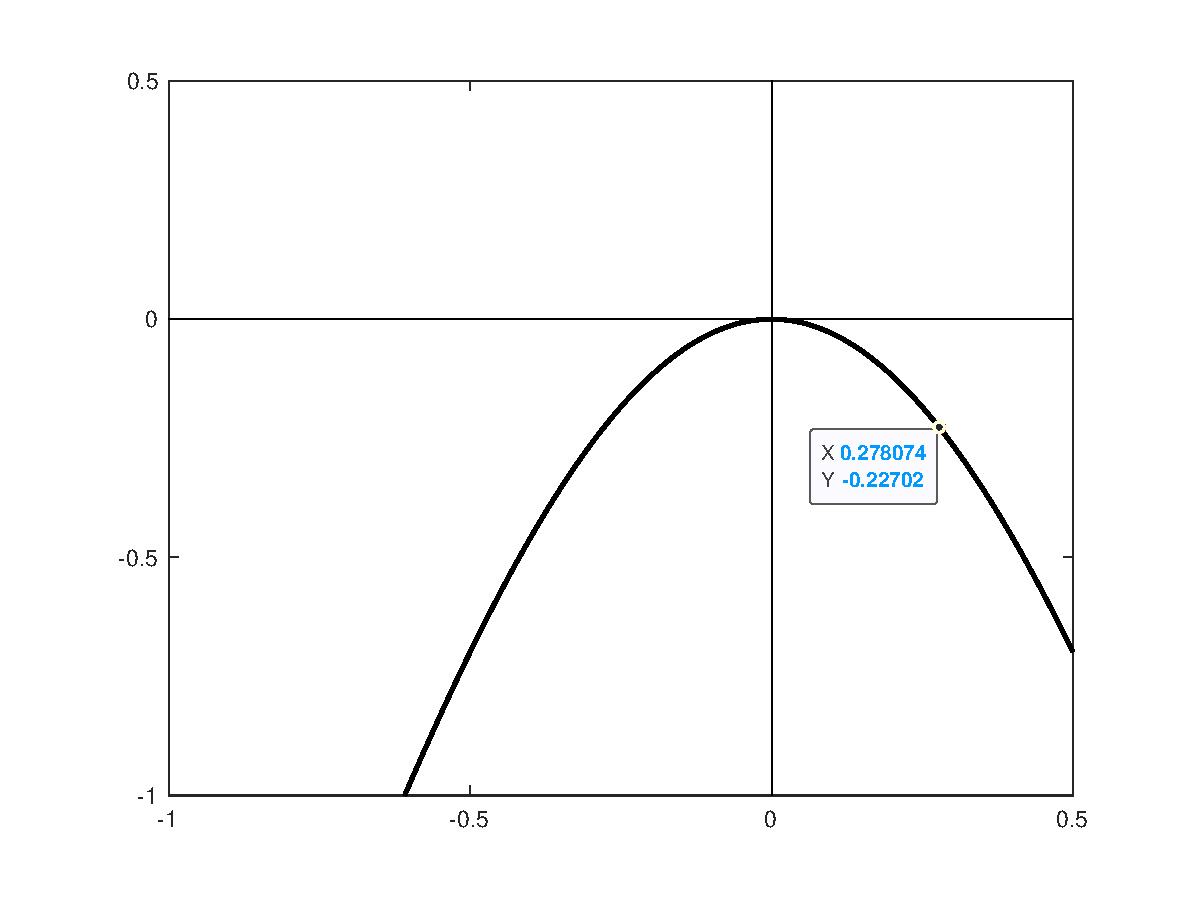
\includegraphics[width=7.5cm]{fig/Q5_d_4.eps}

}
\quad
\subfigure[5(c)]{
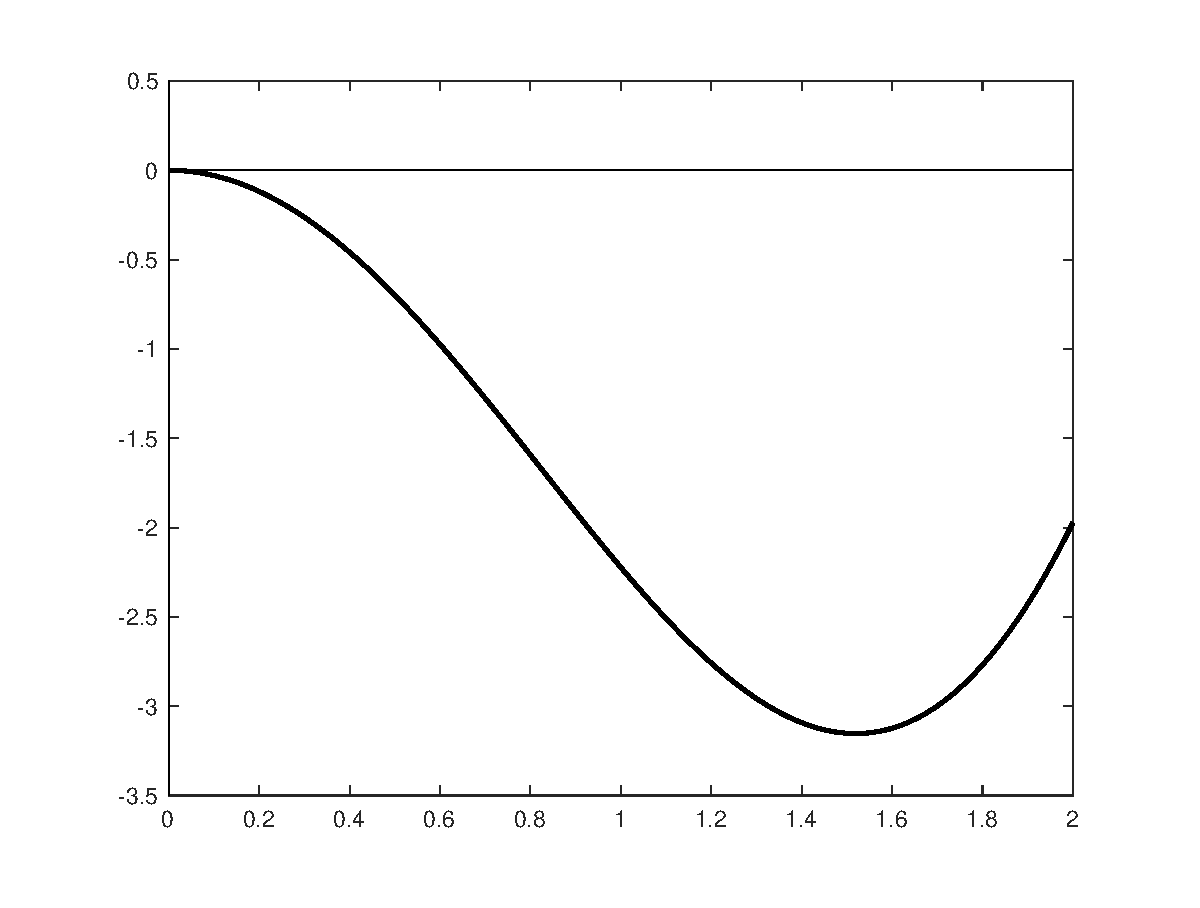
\includegraphics[width=7.5cm]{fig/Q5_d_5.eps}

}

\caption{Function first derivative (slope) diagram}
\label{Q5_d_4}
\end{figure}





To prevent the Root jumping problem when applying the Newton's Method, several tips could be applied to overcome:
\begin{enumerate}
	\item When the function is oscillating or have many roots, The Method of False Position may be a better choice. It has strong stability, but it lags behind in efficiency.
	\item Before iteration, check whether there is a phenomenon that the slope approaches zero near the selected initial point, which will lead to serious deviation of the iterative results in Newton method.
	\item  Choose the point closer to the unknown root as the initial point, which will improve the stability and efficiency of the model to a certain extent.
\end{enumerate}

















	
	
\end{enumerate}


\end{solution}



